\documentclass{beamer}
\usetheme{Berlin}
\usecolortheme{whale}
\usepackage[T1]{fontenc}
\usepackage{lmodern}
\usepackage{booktabs}
\usepackage{tikz}
\setbeamertemplate{navigation symbols}{}

% Edit your thesis details here.
\title[PhD Defence]{Learning Soil Moisture from Sparse Sensors}
\author[J. Lindqvist]{Johanna Lindqvist}
\institute[Dept. of Earth Sciences]{Doctoral Thesis Defence\\Department of Earth Sciences, Halden University}
\date{12 November 2026}

\begin{document}

\begin{frame}
  \titlepage
  \centering\footnotesize
  Supervisor: Prof. M. Ortega \quad Examiners: Dr. K. Baines, Prof. T. Ueda
\end{frame}

\begin{frame}{Roadmap}
  \tableofcontents
\end{frame}

\section{Introduction}
\begin{frame}{The problem}
  \begin{itemize}
    \item Farmers need field scale moisture maps every day.
    \item Satellites are coarse; ground sensors are sparse.
    \item Can we fuse both to get accurate daily maps?
  \end{itemize}
\end{frame}

\begin{frame}{Contributions of this thesis}
  % One block per chapter. Edit titles and text.
  \begin{block}{C1: A sensor fusion model (Chapter 3)}
    Combines satellite and ground data with a spatial prior.
  \end{block}
  \begin{block}{C2: Uncertainty maps (Chapter 4)}
    Tells users where the prediction can be trusted.
  \end{block}
  \begin{block}{C3: Field deployment (Chapter 5)}
    A two season trial on 40 farms.
  \end{block}
\end{frame}

\section{Chapter 3}
\begin{frame}{Fusion model}
  \centering
  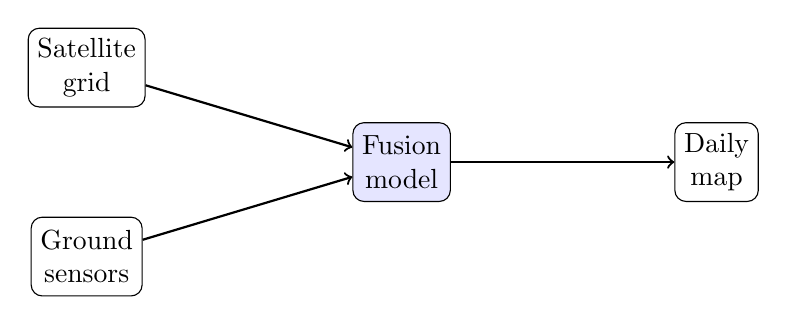
\begin{tikzpicture}[node distance=2cm, every node/.style={draw, rounded corners, align=center, fill=white, minimum height=1cm}]
    \node (sat) at (0,1.2) {Satellite\\grid};
    \node (gnd) at (0,-1.2) {Ground\\sensors};
    \node[fill=blue!10] (m) at (4,0) {Fusion\\model};
    \node (out) at (8,0) {Daily\\map};
    \draw[->, thick] (sat) -- (m);
    \draw[->, thick] (gnd) -- (m);
    \draw[->, thick] (m) -- (out);
  \end{tikzpicture}
\end{frame}

\section{Chapter 4}
\begin{frame}{Uncertainty results}
  \centering
  \begin{tabular}{lcc}
    \toprule
    Region & RMSE & Coverage of 90\% interval \\
    \midrule
    North plain & 0.031 & 0.91 \\
    River valley & 0.044 & 0.88 \\
    Hills & 0.052 & 0.86 \\
    \bottomrule
  \end{tabular}
\end{frame}

\section{Chapter 5}
\begin{frame}{Deployment timeline}
  \centering
  % Move the dots or rename the milestones.
  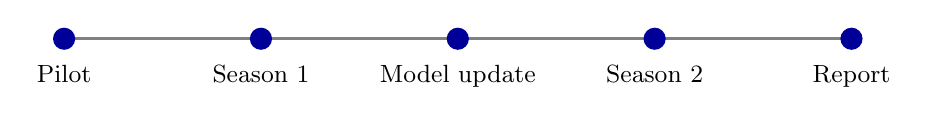
\begin{tikzpicture}
    \draw[very thick, gray] (0,0) -- (10,0);
    \foreach \x/\lab in {0/Pilot, 2.5/Season 1, 5/Model update, 7.5/Season 2, 10/Report} {
      \fill[blue!60!black] (\x,0) circle (4pt);
      \node[below=6pt, font=\small] at (\x,0) {\lab};
    }
  \end{tikzpicture}
  \vspace{1em}
  \begin{itemize}
    \item Irrigation water use fell by 18\% on trial farms.
    \item 34 of 40 farms kept using the maps after the trial.
  \end{itemize}
\end{frame}

\section{Conclusion}
\begin{frame}{Summary and future work}
  \begin{columns}[T]
    \begin{column}{0.48\textwidth}
      \textbf{Summary}
      \begin{itemize}
        \item Accurate daily maps from sparse data.
        \item Honest uncertainty estimates.
        \item Proven in real fields.
      \end{itemize}
    \end{column}
    \begin{column}{0.48\textwidth}
      \textbf{Future work}
      \begin{itemize}
        \item Other crops and climates.
        \item Cheaper sensor placement.
      \end{itemize}
    \end{column}
  \end{columns}
\end{frame}

\begin{frame}{Publications from this thesis}
  \small
  \begin{enumerate}
    \item Lindqvist, J. and Ortega, M. Sensor fusion for soil moisture. \emph{Journal of Hydrology Examples}, 2024.
    \item Lindqvist, J. et al. Calibrated moisture maps. \emph{Proc. Remote Sensing Workshop}, 2025.
    \item Lindqvist, J. et al. A field trial of fused moisture maps. Under review, 2026.
  \end{enumerate}
\end{frame}

\begin{frame}
  \centering\Huge Thank you\\[1em]
  \large Questions from the committee
\end{frame}

\end{document}
